\chapter{FUNDAMENTAÇÃO TEÓRICA}\label{fund}
Neste capítulo serão descritos as bases de todos os conhecimentos utilizados para o desenvolvimento deste projeto.
\section{Seção 1}\label{label1}

descrição geral da seção 1

\subsection{Subseção 1}\label{labelS1}


\subsection{subseção 2}

Modelo de tabela.

\begin{table}[htbp!]
  \centering
    \caption{título da tabela}
      \begin{tabularx}{\textwidth}{|X|X|X|}
      \hline
      \textbf{Texto} &  \textbf{Texto} & \textbf{Texto} \\
      \hline
      Texto1 & Texto2 & Texto3 \\
      \hline
      \end{tabularx}
  \label{Tabela1}
\end{table}
% \pagebreak

\subsection{subseção 3}\label{labels3}
Exemplo de inserção de figura

\begin{figure}[htp!]
\centering
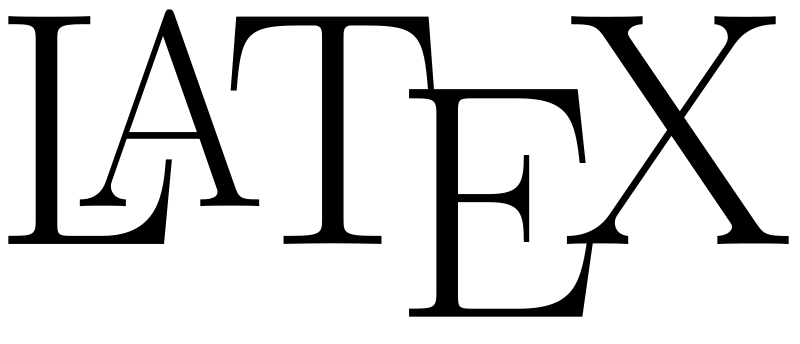
\includegraphics[width=0.80\textwidth]{figuras/latex.png}
\caption{Nome da Figura}
\label{figura1}
\end{figure}
\pagebreak

\section{Seção 2}
Exemplo de citação:

\begin{citacao}
``O raciocínio baseado em casos (RBC) é um enfoque para a solução de problemas e para o aprendizado baseado em experiência passada. RBC resolve problemas ao recuperar e adaptar experiências passadas – chamadas casos – armazenadas em uma base de casos. Um novo problema é resolvido com base na adaptação de soluções de problemas similares já conhecidos.'' \cite{wang}
\end{citacao}


